\section{Rotar canales}
\par{El filtro consiste en una rotación de canales en cada píxel, como bien indica su nombre. Y la rotación se da de esta manera:}
\begin{center}
\textbf{R} $\longrightarrow$ \textbf{G}\\
\textbf{G} $\longrightarrow$ \textbf{B}\\
\textbf{B} $\longrightarrow$ \textbf{R}\\
\end{center}

\subsection{Código C}
\par{En el código de C recorremos la matriz iterando sus filas y columnas y modificando un píxel a la vez.
A continuación presentamos su pseudocódigo}

\begin{algorithm}[h!]
\caption{Rotar}
\begin{algorithmic}
  \Function{rotar}{src: *unsigned char, dst: *unsigned char, cols: int, filas: int, srcRowSize: int, dstRowSize: int}
	\State $unsigned~ char~ (*srcMatrix)[srcRowSize] = (unsigned~ char (*)[srcRowSize])~ src$
	\State $unsigned~ char~ (*dstMatrix)[dstRowSize] = (unsigned~ char (*)[dstRowSize])~ dst$
	\For{$f \gets 0~..~filas-1$}
		\For{$c \gets 0~..~cols-1$}
			\State $bgra_t* p_s \gets (bgra_t*)$ \& $srcMatrix[f][c * 4]$
			\State $bgra_t *p_d \gets (bgra_t*)$ \&$dstMatrix[f][c * 4]$
			
			\State $p_d \rightarrow$b $\gets$ $p_s \rightarrow g$
			\State $p_d \rightarrow$g $\gets$ $p_s \rightarrow r$
			\State $p_d \rightarrow$r $\gets$ $p_s \rightarrow b$
			\State $p_d \rightarrow$ a $\gets$ $p_s \rightarrow a$
		\EndFor
	\EndFor
\EndFunction
\end{algorithmic} 
\end{algorithm}
	
\subsection{Código ASM}
\par{El código de ASM recorre la matriz de la misma manera que la recorre el código de C, pero procesa 4 píxeles por iteración.}
\par{Las instrucciones propias de SIMD aceleran mucho el proceso y aportan mejoras considerables incluso al compararlo con un código de ASM sin utilizarlas.}

En cada ciclo se cargan 4 píxeles en xmm0 y se aplica \textbf{pshufb xmm0, xmm3}, donde este es:
\xmmb{$0f$}{$0c$}{$0e$}{$0d$}{$0b$}{$08$}{$0a$}{$09$}{$07$}{$04$}{$06$}{$05$}{$03$}{$00$}{$02$}{$01$}
Luego se guarda en memoria en la imagen destino, se incrementa el contador en 4 (procesamos 4 píxeles) y los respectivos punteros a las imagenes en 16 (4 píxeles ocupan 16 bytes).	
	
	
\subsection{Experimentación}

\subsubsection{Idea}	
\par{Para la experimentación con Rotar notamos la facilidad con la que se codea y procesa el filtro gracias a las instrucciones de SIMD, por ello quisimos ver si, además, generaban alguna optimización sobre un código sin estas herramientas.}
\par{Luego comparamos la eficiencia de ASM contra el código de C y distintas optimizaciones de este.}

\subsubsection{Hipótesis}
\par{La hipótesis que tuvimos sobre la primera idea era que efectivamente íbamos a notar un cambio ya que íbamos a estar procesando la mitad de píxeles por iteración. También suponíamos que iba a ser más complicado manipular los píxeles al no contar con instrucciones como \textbf{shuffle}, \textbf{unpacked}, \textbf{psrlx} y \textbf{psllx}.}
	
\subsubsection{Resultados}
\par{Efectivamente vimos una notoria diferencia entre el código en ASM con y sin SIMD, más aún, el código optimizado de C es más eficiente que éste último.}
\par{A continuación adjuntamos un gráfico en el que se puede apreciar dicha diferencia.}
	
\begin{figure}[H]
\centering
\captionsetup{justification=centering}
	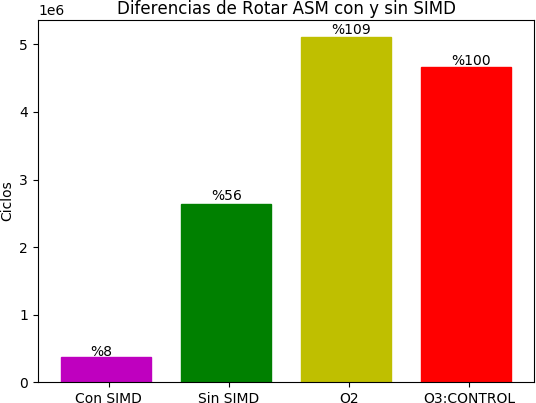
\includegraphics[width = 12 cm, height = 8 cm]{imagenes/SinSIMD.png}
\caption[center]{Gráfico que compara las velocidad de las ejecuciones de las implementaciones con y sin el uso de instrucciones SSE, y también con optimizaciones de la implementación en C.}
\end{figure}

\par{El gráfico se armó en base a un conjunto de corridas de cada implementación del filtro, de donde se tomó la cantidad mínima de ciclos; con esto buscamos reducir la proporción de tiempo que consideramos que nuestro programa no estaba corriendo, si no que el scheduler estaba ejecutando otro programa.}\\
\par{A continuación mostramos un gráfico (armado de igual manera que el anterior) donde mostramos los tiempos de ejecución del filtro implementado en ASM y en C con distintas optimizaciones.}
	
\begin{figure}[H]
\centering
\captionsetup{justification=centering}
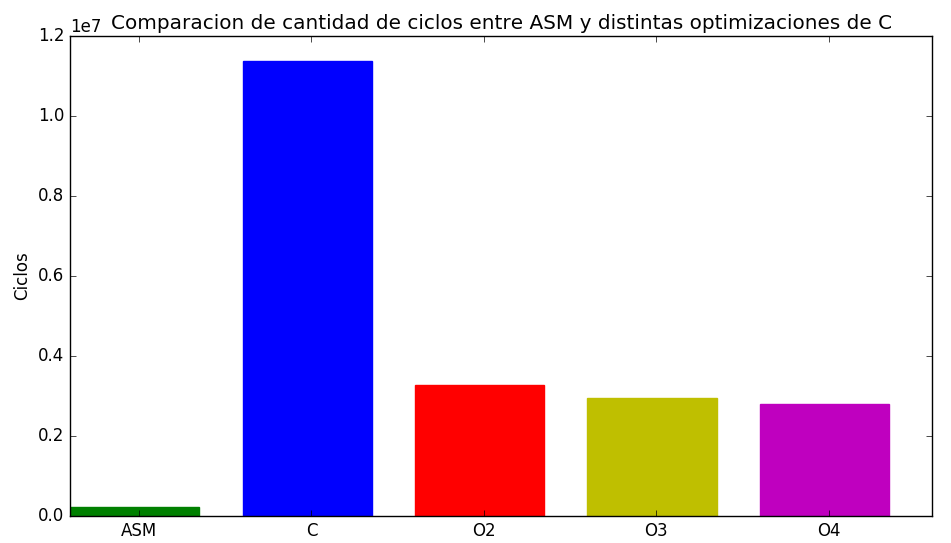
\includegraphics[width = 13 cm, height = 8 cm]{imagenes/rotarConC.png}
\caption[center]{Diferencias en cantidad de ciclos para la ejecución del filtro con la implementación en ASM y la de C con sus optimizaciones.}
\end{figure}